\subsection{Utente non autenticato}
\subsubsection{Panoramica utente non autenticato}
\begin{figure}[H]
\centering
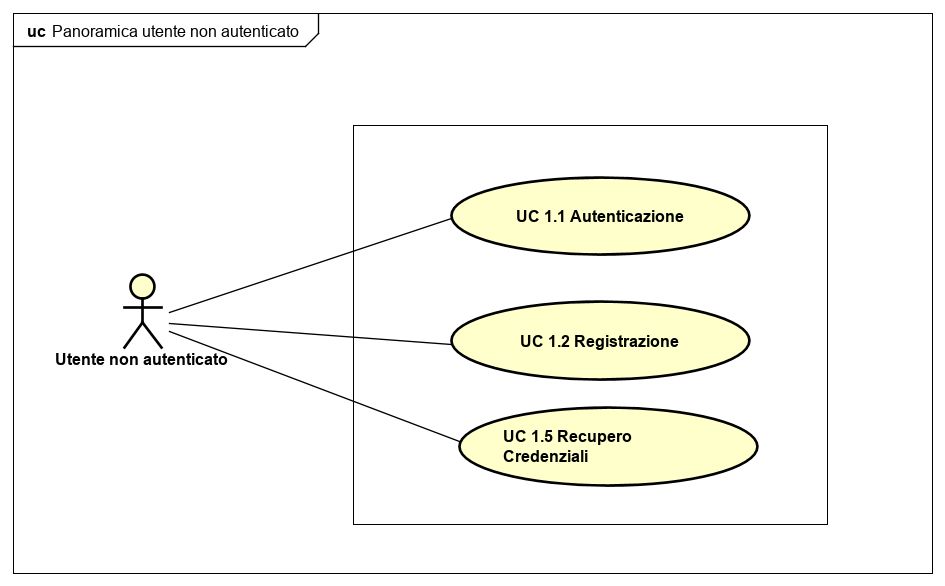
\includegraphics[width=17cm]{img/UC1.png} 
\caption{Panoramica utente non autenticato}\label{fig:1}
\end{figure}


\subsubsection{UC 1.1 - Autenticazione}

\begin{figure}[H]
\centering
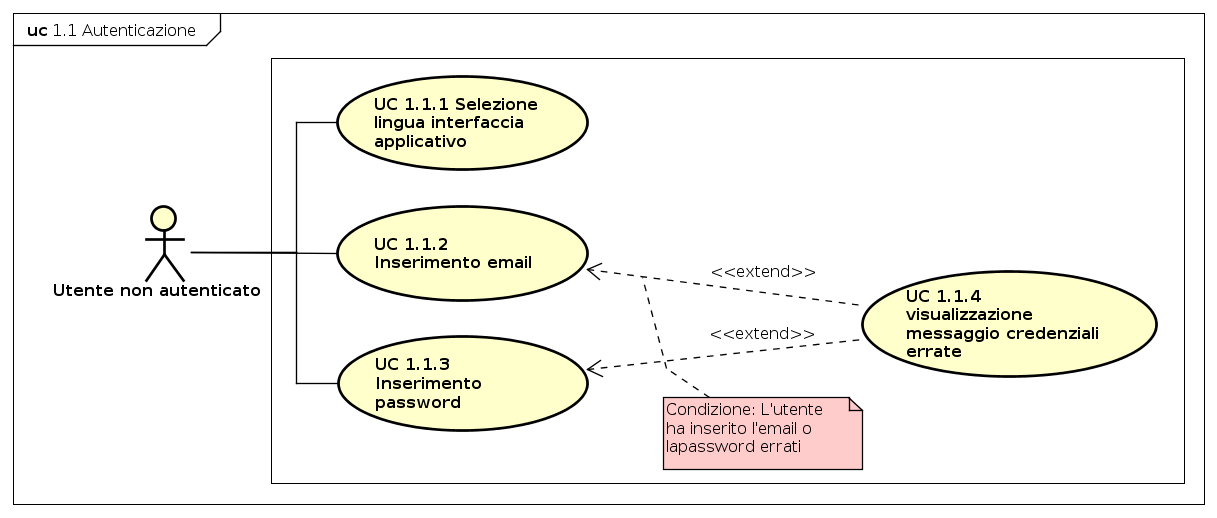
\includegraphics[width=17cm]{img/UC11.png} 
\caption{Caso d'uso UC 1.1}
\end{figure}

\begin{itemize}
\item[•]\textbf{Attori}: Utente non autenticato;
\item[•]\textbf{Descrizione}:  l’utente non identificato inserisce username e password e si autentica accedendo alla dashboard;
\item[•]\textbf{Precondizione}: l’utente non è autenticato;
\item[•]\textbf{Postcondizione}: l’utente viene autenticato all’interno del sistema;
\item[•]\textbf{Flusso degli eventi}:
\begin{enumerate}
\item UC 1.1.1 - Inserimento nome utente;
\item UC 1.1.2 - Inserimento password;

\end{enumerate}
\item[•]\textbf{Estensioni}:
\begin{enumerate}
\item UC 1.1.3 - visualizzazione messaggio credenziali errate;
\end{enumerate}
\end{itemize}

\subsubsection{UC 1.1.1 - Inserimento nome utente}
\begin{itemize}
\item[•]\textbf{Attori}: Utente non autenticato;
\item[•]\textbf{Descrizione}: l’utente inserisce un nome utente durante l'autenticazione;
\item[•]\textbf{Precondizione}: l’utente non è autenticato;
\item[•]\textbf{Postcondizione}: l’utente ha inserito il proprio nome utente;
\item[•]\textbf{Flusso degli eventi}: l'utente visualizza il form per l'autenticazione e inserisce il nome utente in un apposito campo.

\end{itemize}

\subsubsection{UC 1.1.2 - Inserimento password}
\begin{itemize}
\item[•]\textbf{Attori}: Utente non autenticato;
\item[•]\textbf{Descrizione}: l’utente inserisce una password;
\item[•]\textbf{Precondizione}: l'utente non è autenticato;
\item[•]\textbf{Postcondizione}: l'utente ha inserito la propria password;
\item[•]\textbf{Flusso degli eventi}: l'utente visualizza il form per l'autenticazione e inserisce la password in apposito campo.
\end{itemize}

\subsubsection{UC 1.1.3 - Visualizzazione messaggio credenziali errate}
\begin{itemize}
\item[•]\textbf{Attori}: Utente non autenticato;
\item[•]\textbf{Descrizione}: l'utente ha avviato il login immettendo delle credenziali errati;
\item[•]\textbf{Precondizione}: l'utente non è autenticato;
\item[•]\textbf{Postcondizione}: l'utente riceve il messaggio d'errore per aver inserito username o password errati;
\item[•]\textbf{Flusso degli eventi}: l'utente visualizza il form per l'autenticazione, inserisce nome utente e password in appositi campi, riscontrando errore sulle credenziali.
\end{itemize}

\subsubsection{UC 1.2 - Registrazione utente}
\begin{figure}[H]
	\centering
	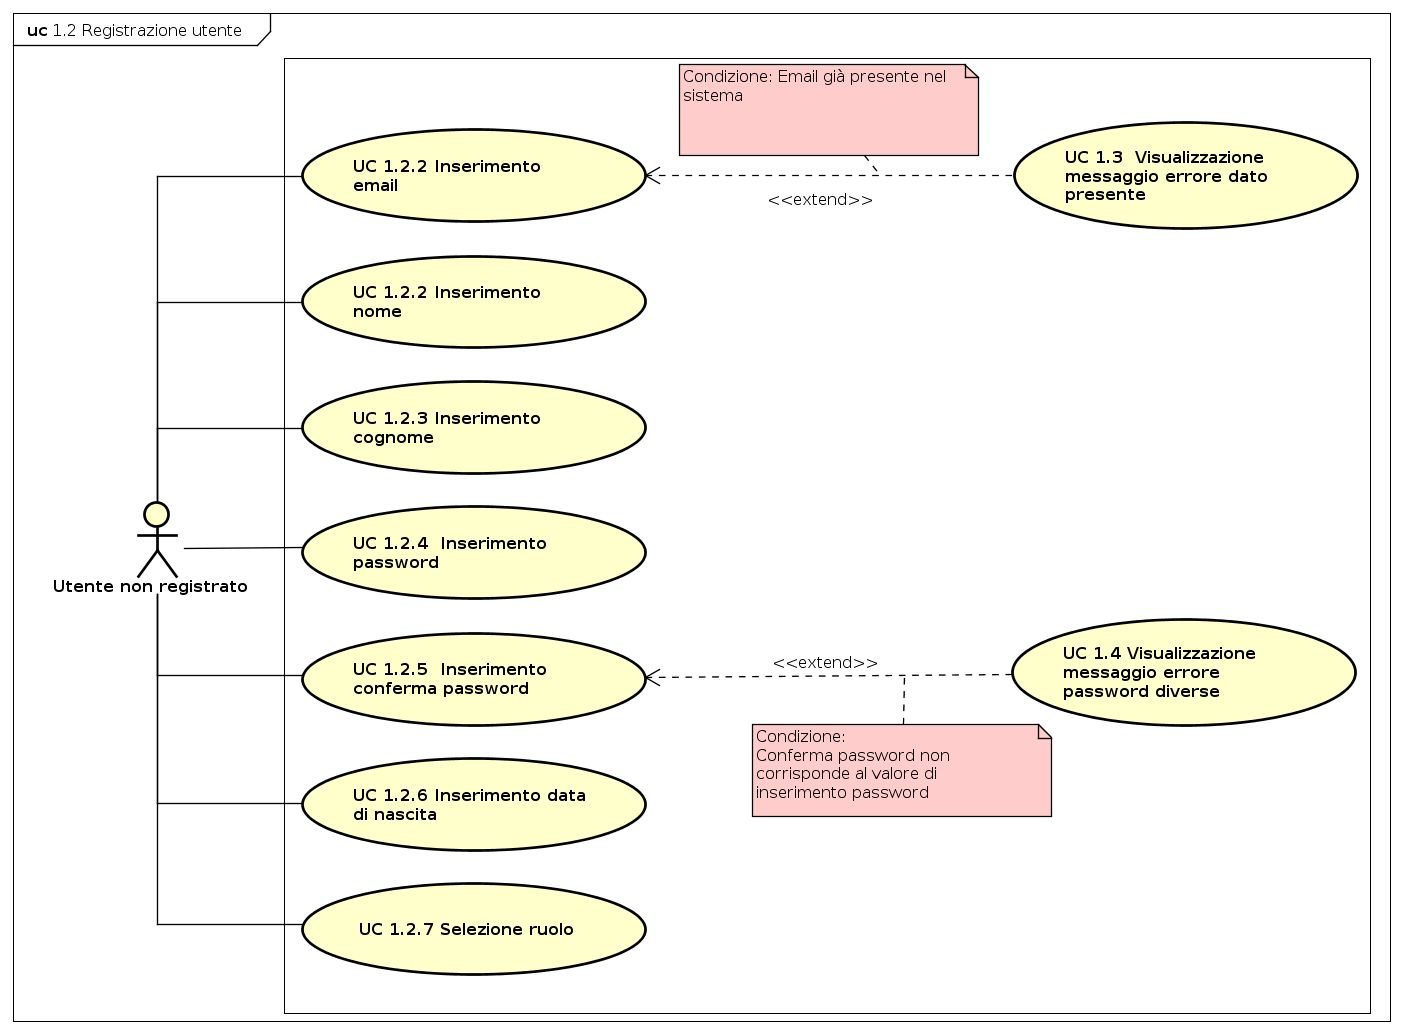
\includegraphics[width=17cm]{img/UC12.png} 
	\caption{Caso d'uso UC 1.2}\label{fig:12}
\end{figure}
\begin{itemize}
	\item[•]\textbf{Attori}: Utente non autenticato;
	\item[•]\textbf{Descrizione}: l'utente non autenticato compila il modulo di registrazione al fine di poter accedere al sistema;
	\item[•]\textbf{Precondizione}: l'utente non è autenticato;
	\item[•]\textbf{Postcondizione}: l'utente si è registrato e può quindi accedere al sistema;
	\item[•]\textbf{Flusso degli eventi}:
	\begin{enumerate}
		\item UC 1.2.1 - Inserimento nome utente;
		\item UC 1.2.2 - Inserimento email;
		\item UC 1.2.3 - Inserimento password;
		\item UC 1.2.4 - Inserimento conferma password;
		\item UC 1.2.5 - Inserimento data di nascita;
		\item UC 1.2.6 - Selezione ruolo;
		\item UC 1.2.7 - Inserimento nome;
		\item UC 1.2.8 - Inserimento cognome;
		\item UC 1.2.9 - Selezione lingua applicativo.	
	\end{enumerate}
	\item[•]\textbf{Estensioni}:
	\begin{enumerate}
		\item UC 1.3 - Visualizzazione messaggio errore dato presente;
		\item UC 1.4 - Visualizzazione messaggio errore password diverse.
	\end{enumerate}
\end{itemize}

\subsubsection{UC 1.2.1 - Inserimento nome utente}
\begin{itemize}
	\item[•]\textbf{Attori}: Utente non autenticato;
	\item[•]\textbf{Descrizione}: l'utente inserisce un nome utente durante la registrazione;
	\item[•]\textbf{Precondizione}: l'utente non è autenticato e il nome utente non è definito;
	\item[•]\textbf{Postcondizione}: l'utente ha inserito un nome utente;
	\item[•]\textbf{Flusso degli eventi}: l'utente visualizza il form per la registrazione e inserisce il nome utente in un apposito campo.
	\item[•] \textbf{Estensioni}:
	\begin{enumerate}
		\item UC 1.3 - Visualizzazione messaggio errore dato presente.
	\end{enumerate}
\end{itemize}

\subsubsection{UC 1.2.2 - Inserimento e-mail}
\begin{itemize}
	\item[•]\textbf{Attori}: Utente non autenticato;
	\item[•]\textbf{Descrizione}: l'utente inserisce la sua email durante la registrazione;
	\item[•]\textbf{Precondizione}: l'utente non è autenticato e la email non è definita;
	\item[•]\textbf{Postcondizione}: l'utente ha inserito la propria email;
	\item[•]\textbf{Flusso degli eventi}: l'utente visualizza il form per la registrazione e inserisce la propria e-mail in apposito campo.
	\item[•] \textbf{Estensioni}:
		\begin{enumerate}
		\item UC 1.3 - Visualizzazione messaggio errore dato presente.
	\end{enumerate}
\end{itemize}

\subsubsection{UC 1.2.3 - Inserimento password}
\begin{itemize}
	\item[•]\textbf{Attori}: Utente non autenticato;
	\item[•]\textbf{Descrizione}: l'utente inserisce una password durante procedura di registrazione;
	\item[•]\textbf{Precondizione}: l'utente non è autenticato e la password non è definita;
	\item[•]\textbf{Postcondizione}: l'utente ha inserito una password;
	\item[•]\textbf{Flusso degli eventi}:l'utente visualizza il form per la registrazione e inserisce la propria password in apposito campo.
	\item[•] \textbf{Estensioni}:
	\begin{enumerate}
		\item UC 1.4 - Visualizzazione messaggio errore password diverse.
	\end{enumerate}
\end{itemize}

\subsubsection{UC 1.2.4 - Inserimento conferma password}
\begin{itemize}
	\item[•]\textbf{Attori}: Utente non autenticato;
	\item[•]\textbf{Descrizione}: l'utente inserisce la conferma della password durante la registrazione;
	\item[•]\textbf{Precondizione}: l'utente non è autenticato e la conferma password non è definita;
	\item[•]\textbf{Postcondizione}: l'utente ha inserito la conferma della password;
	\item[•]\textbf{Flusso degli eventi}: l'utente visualizza il form per la registrazione e inserisce, confermando per la seconda volta, la propria password in un apposito campo e conferma la password.
	\item[•] \textbf{Estensioni}:
		\begin{enumerate}
		\item UC 1.4 - Visualizzazione messaggio errore password diverse.
	\end{enumerate}
\end{itemize}

\subsubsection{UC 1.2.5 - Inserimento data di nascita}
\begin{itemize}
	\item[•]\textbf{Attori}: Utente non autenticato;
	\item[•]\textbf{Descrizione}: l'utente inserisce la sua data di nascita durante la registrazione;
	\item[•]\textbf{Precondizione}: l'utente non è autenticato e la data di nascita non è definita;
	\item[•]\textbf{Postcondizione}: l'utente ha inserito la sua data di nascita;
	\item[•]\textbf{Flusso degli eventi}: l'utente visualizza il form per la registrazione e inserisce la data di nascita in un apposito campo.
\end{itemize}

\subsubsection{UC 1.2.6 - Selezione ruolo}
\begin{itemize}
	\item[•]\textbf{Attori}: Utente non registrato;
	\item[•]\textbf{Descrizione}: l'utente seleziona il ruolo che vorrebbe ricoprire all'interno dell'applicativo;
	\item[•]\textbf{Precondizione}: l'utente non è registrato e il ruolo non è definito;
	\item[•]\textbf{Postcondizione}: l'utente ha inserito il ruolo desiderato;
	\item[•]\textbf{Flusso degli eventi}:l'utente non registrato seleziona la scelta del ruolo tra: allievo, insegnante e sviluppatore.
\end{itemize}

\subsubsection{UC 1.2.7 - Inserimento nome}
\begin{itemize}
\item[•]\textbf{Attori}: Utente non autenticato;
\item[•]\textbf{Descrizione}: l'utente inserisce il suo nome durante la registrazione;
\item[•]\textbf{Precondizione}: l'utente non è autenticato e il nome non è definito;
\item[•]\textbf{Postcondizione}: l'utente ha inserito il suo nome;
\item[•]\textbf{Flusso degli eventi}: l'utente visualizza il form per la registrazione e inserisce il suo nome in un apposito campo.
\end{itemize}

\subsubsection{UC 1.2.8 - Inserimento cognome}
\begin{itemize}
	\item[•]\textbf{Attori}: Utente non autenticato;
	\item[•]\textbf{Descrizione}: l'utente inserisce il suo cognome durante la registrazione;
	\item[•]\textbf{Precondizione}: l'utente non è autenticato e il cognome non è definito;
	\item[•]\textbf{Postcondizione}: l'utente ha inserito il suo cognome;
	\item[•]\textbf{Flusso degli eventi}: l'utente visualizza il form per la registrazione e inserisce il suo cognome in un apposito campo.
\end{itemize}

\subsubsection{UC 1.3 - Visualizzazione messaggio errore dato presente}
\begin{itemize}
	\item[•]\textbf{Attori}: Utente non registrato;
	\item[•]\textbf{Descrizione}: l'utente non registrato visualizza un messaggio di errore relativo all'inserimento
	di un dato già presente nel sistema;
	\item[•]\textbf{Precondizione}: l'utente non registrato sta completando la procedura di registrazione;
	\item[•]\textbf{Postcondizione}: l'utente visualizza un messaggio di errore relativo all'inserimento di un valore già presente nel sistema;
	\item[•]\textbf{Flusso degli eventi}: l'utente inserisce una email o un nome utente già presente nel sistema, pertanto riceve un messaggio di errore.
\end{itemize}

\subsubsection{UC 1.4 - Visualizzazione messaggio errore password diverse}
\begin{itemize}
	\item[•]\textbf{Attori}: Utente non registrato;
	\item[•]\textbf{Descrizione}: l'utente non registrato visualizza un messaggio che comunica che i valori della password e di conferma password sono tra loro diversi;
	\item[•]\textbf{Precondizione}: l'utente non registrato ha inserito la password e la conferma password con valori differenti;
	\item[•]\textbf{Postcondizione}: l'utente visualizza un messaggio di errore relativo all'inserimento di password e conferma password con valori diversi;
	\item[•]\textbf{Flusso degli eventi}: l'utente inserisce password e conferma password con valori diversi, pertanto riceve un messaggio di errore.
\end{itemize}

\subsubsection{UC 1.5 - Recupero Credenziali}
\begin{itemize}
	\item[•]\textbf{Attori}: Utente non autenticato;
	\item[•]\textbf{Descrizione}: l’utente avvia iter per il recupero delle proprie credenziali smarrite;
	\item[•]\textbf{Precondizione}: l’utente non è autenticato;
	\item[•]\textbf{Postcondizione}: l’utente ha inviato la richiesta di recupero;
	\item[•]\textbf{Flusso degli eventi}:
	l’utente avvia iter per il recupero delle proprie credenziali, inserisce la propria email e invia una richiesta.
\end{itemize}